\documentclass[a4paper]{article}


%use the english line for english reports
%usepackage[english]{babel}
\usepackage[portuguese]{babel}
\usepackage{indentfirst}
\usepackage{graphicx}
\usepackage{verbatim}
\usepackage{fancyhdr} % Required for custom headers
\usepackage{lastpage} % Required to determine the last page for the footer
\usepackage{extramarks} % Required for headers and footers
\usepackage[usenames,dvipsnames]{color} % Required for custom colors
\usepackage{graphicx} % Required to insert images
\usepackage{listings} % Required for insertion of code
\usepackage{courier} % Required for the courier font
\usepackage{lipsum} % Used for inserting dummy 'Lorem ipsum' text into the template
\RequirePackage[T1]{fontenc}
\RequirePackage[utf8]{inputenc}


\begin{document}

\setlength{\textwidth}{16cm}
\setlength{\textheight}{22cm}

\title{\Huge\textbf{Morelli}\linebreak\linebreak\linebreak
\Large\textbf{Relatório Intercalar}\linebreak\linebreak
\linebreak\linebreak

\includegraphics[scale=0.1]{feup-logo.png}\linebreak\linebreak
\linebreak\linebreak
\Large{Mestrado Integrado em Engenharia Informática e Computação} \linebreak\linebreak
\Large{Programação em Lógica}\linebreak
}

\author{\textbf{Grupo Morelli3: }\\
Francisco Rodrigues - 201305627 \\
Marta Lopes - 201208067 \\
\linebreak\linebreak \\
 \\ Faculdade de Engenharia da Universidade do Porto \\ Rua Roberto Frias, s\/n, 4200-465 Porto, Portugal \linebreak\linebreak\linebreak
\linebreak\linebreak\vspace{1cm}}

\maketitle

\thispagestyle{empty}

%************************************************************************************************
%************************************************************************************************

\newpage

%Todas as figuras devem ser referidas no texto. %\ref{fig:codigoFigura}
%
%%Exemplo de código para inserção de figuras
%%\begin{figure}[h!]
%%\begin{center}
%%escolher entre uma das seguintes três linhas:
%%\includegraphics[height=20cm,width=15cm]{path relativo da imagem}
%%\includegraphics[scale=0.5]{path relativo da imagem}
%%\includegraphics{path relativo da imagem}
%%\caption{legenda da figura}
%%\label{fig:codigoFigura}
%%\end{center}
%%\end{figure}
%
%
%\textit{Para escrever em itálico}
%\textbf{Para escrever em negrito}
%Para escrever em letra normal
%``Para escrever texto entre aspas''
%
%Para fazer parágrafo, deixar uma linha em branco.
%
%Como fazer bullet points:
%\begin{itemize}
	%\item Item1
	%\item Item2
%\end{itemize}
%
%Como enumerar itens:
%\begin{enumerate}
	%\item Item 1
	%\item Item 2
%\end{enumerate}
%
%\begin{quote}``Isto é uma citação''\end{quote}

%%%%%%%%%%%%%%%%%%%%%%%%%%
%----------------------------------------------------------------------------------------
%	TABLE OF CONTENTS
%----------------------------------------------------------------------------------------

%\setcounter{tocdepth}{1} % Uncomment this line if you don't want subsections listed in the ToC

\newpage
\tableofcontents
\newpage

\section{Descrição do Jogo}
%%%%%%%%%%%%%%%%%%%%%%%%%%
\subsection{História}

\textit{Morelli} é um jogo de tabuleiro criado por \textit{Richar Moxham} em 2011. É jogado por apenas 2 jogadores num tabuleiro preferencialmente de 13x13 quadrados coloridos em faixas concêntricas (Fig.1). A faixa de fora será a maior, com 48 casas vermelhas, depois o laranja, amarelo, verde, azul, roxo e terminando na casa central em violeta. 


\begin{center}
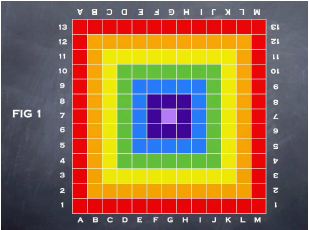
\includegraphics[scale=0.9]{fig1.png}\linebreak\linebreak 
\end{center}


%%%%%%%%%%%%%%%%%%%%%%%%%%
\newpage
\subsection{Regras de Jogo}

\begin{itemize}
	\item O jogo começa com \textbf{24 peças pretas} e \textbf{24 peças brancas}, ambas reversíveis, posicionadas nos quadrados vermelhos, de forma diametralmente oposta. Podem estar de frente umas para as outras (Fig.2), adjacentes (Fig.3) ou soltas (Fig.4). Para além disso cada jogador vai ter \textbf{uma torre da cor respectiva}, que não vai entrar no tabuleiro no inicio do jogo. 
\begin{center}
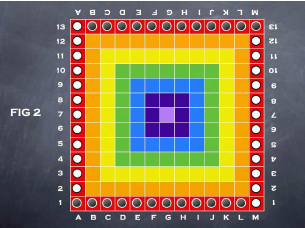
\includegraphics[scale=0.9]{fig2.png}\linebreak\linebreak 
\end{center}

\begin{center}
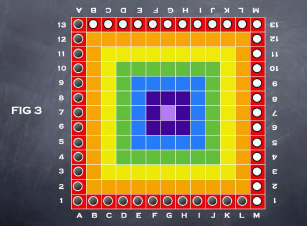
\includegraphics[scale=0.9]{fig3.png}\linebreak\linebreak 
\end{center}

\begin{center}
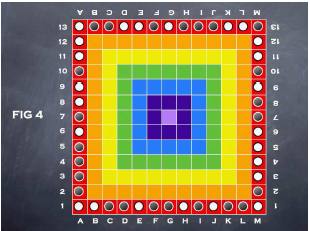
\includegraphics[scale=0.9]{fig4.png}\linebreak\linebreak 
\end{center}

	\item Cada jogador joga na sua vez, começando primeiro o jogador que tiver as peças da cor preta. Um \textbf{movimento legal} (Fig.5) consiste em mover a peça para um quadrado desocupado numa linha ortogonal ou diagonal desde que seja para uma faixa de cor mais próxima do centro do que aquela em que se encontra no momento, não se podendo manter na mesma faixa ou voltar para trás (Fig.6).

\begin{center}
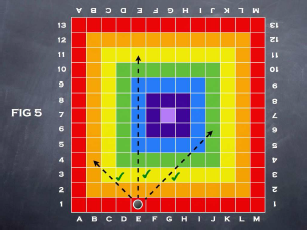
\includegraphics[scale=0.9]{fig5.png}\linebreak\linebreak 
\end{center}

\begin{center}
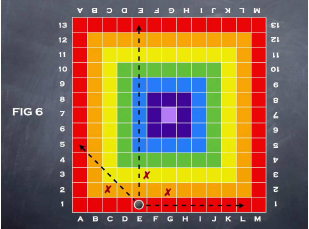
\includegraphics[scale=0.9]{fig6.png}\linebreak\linebreak 
\end{center}
	
	\newpage
	\item Apenas será possivel passar pelo centro se este estiver vazio, não podendo parar nele. (Fig.7, Fig.8).


\begin{center}
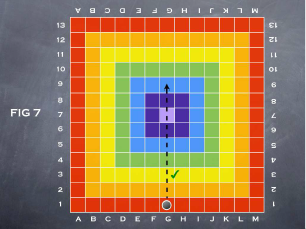
\includegraphics[scale=0.9]{fig7.png}\linebreak\linebreak 
\end{center}

\begin{center}
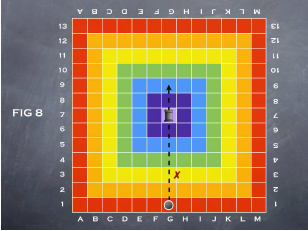
\includegraphics[scale=0.9]{fig8.png}\linebreak\linebreak 
\end{center}
	\newpage
	\item A \textbf{captura do centro} é feita quando o jogador cria um quadrado de qualquer tamanho com as suas peças, centrado na célula central (Fig.9, Fig. 10, Fig. 11). Quando o centro está capturado é colocada a torre da cor respectiva no centro do tabuleiro, removendo a torre adversária se se aplicar.

\begin{center}
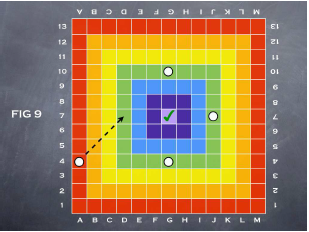
\includegraphics[scale=0.9]{fig9.png}\linebreak\linebreak 
\end{center}

\begin{center}
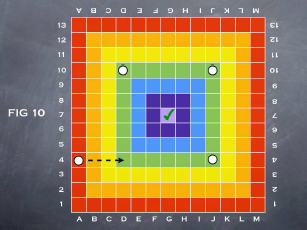
\includegraphics[scale=0.9]{fig10.png}\linebreak\linebreak 
\end{center}

\begin{center}
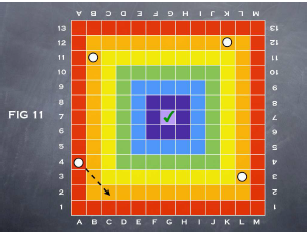
\includegraphics[scale=0.9]{fig11.png}\linebreak\linebreak 
\end{center}

	\item A cada movimento o jogador poderá \textbf{capturar uma peça adversária} quando conseguir rodea-la por duas peças da sua cor seja ortogonal ou diagonalmente (Fig.12). Uma peça capturada é revertida passando para a cor contrária. 

\begin{center}
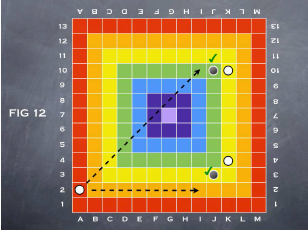
\includegraphics[scale=0.9]{fig12.png}\linebreak\linebreak 
\end{center}

	\item O \textbf{vencedor} será o jogador que terá a sua torre no centro no final do jogo. O jogo acaba quando não existirem mais jogadas possíveis ou, se for um jogo cronometrado, quando o tempo acabar. Se o centro se mantiver sem nenhuma torre até ao final do jogo, é um empate. 
	
\end{itemize}
\newpage

\newpage
\section{Representação e visualização do Estado de Jogo}


\begin{center}

\textbf{P: Peças pretas} \linebreak\linebreak
\textbf{W: Peças brancas} \linebreak\linebreak
\textbf{WT: Torre branca} \linebreak\linebreak
\textbf{N: Centro vazio} \linebreak\linebreak

\end{center}
\textbf{Representação do estado inicial do tabuleiro:}
\begin{center}
\hspace*{-2cm}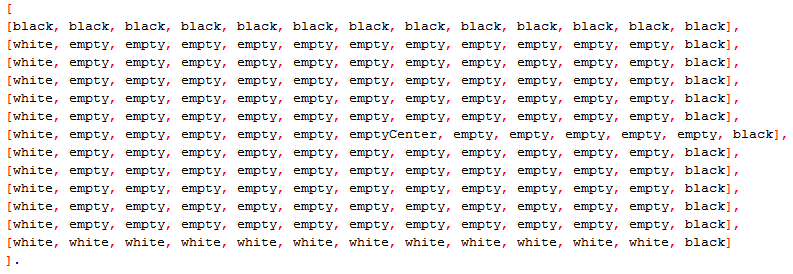
\includegraphics[scale=0.85]{gameex1rep.png}\linebreak\linebreak

    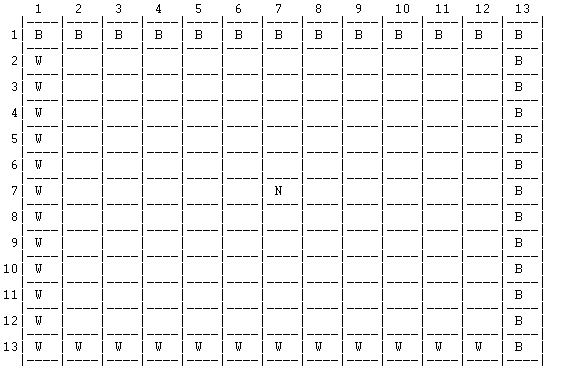
\includegraphics[scale=0.9]{gameex1.png}\linebreak
Figura 13: Estado inicial do tabuleiro visualizado na consola \linebreak\linebreak\linebreak

\end{center}
\textbf{Representação de um estado intermédio do tabuleiro:}
\begin{center}
\hspace*{-2cm}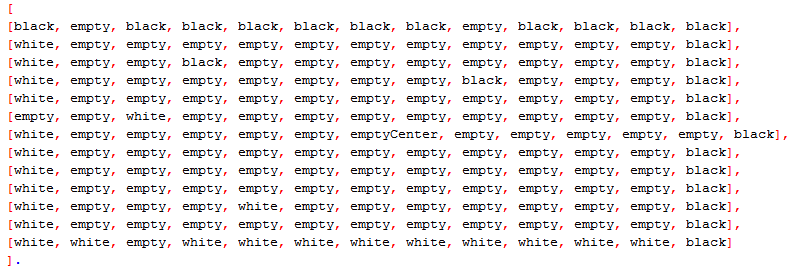
\includegraphics[scale=0.85]{gameex2rep.png}\linebreak\linebreak
 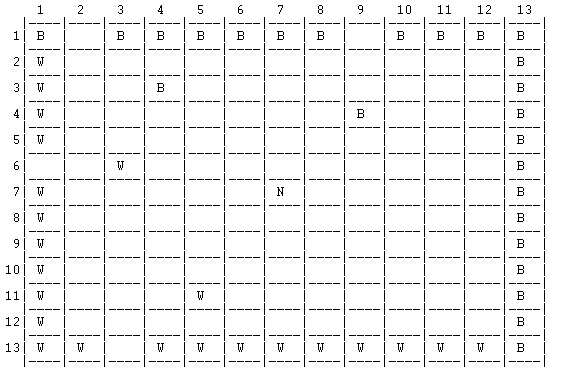
\includegraphics[scale=0.9]{gameex2.png}\linebreak
Figura 14: Possivel estado intermédio de jogo \linebreak\linebreak\newpage

\end{center}
\textbf{Representação de um estado final do tabuleiro:}
\begin{center}
\hspace*{-2cm}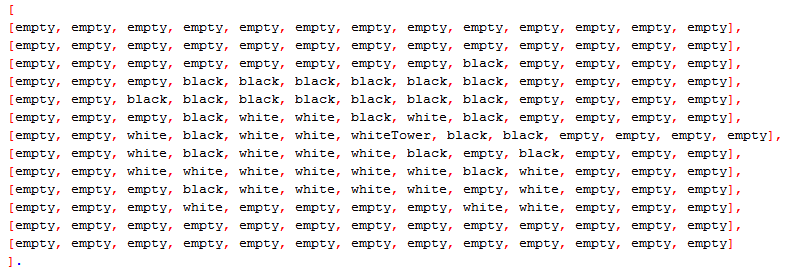
\includegraphics[scale=0.85]{gameex3rep.png}\linebreak\linebreak
 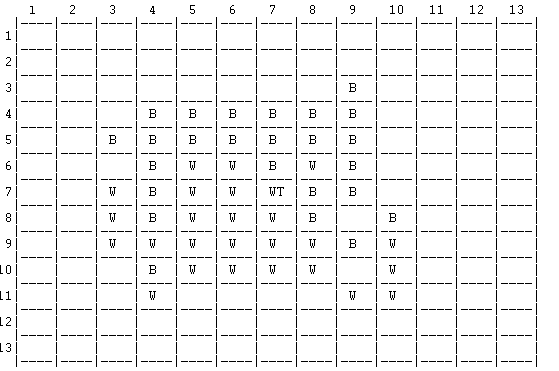
\includegraphics[scale=0.9]{gameex3.png}\linebreak
Figura 15: Possivel estado final de jogo com o centro capturado pelos brancos \linebreak\linebreak
\end{center}

\subsection{Código usado para a estrutura do tabuleiro}

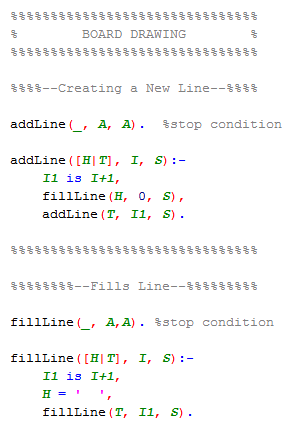
\includegraphics[scale=1]{code1.png}\linebreak


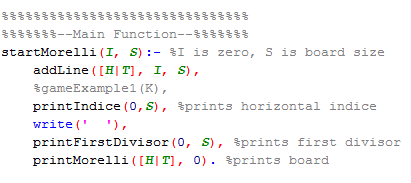
\includegraphics[scale=1]{code2.png}\linebreak\linebreak

\newpage
\section{Movimentos}
\subsection{Cabeçalho do predicado de movimentação de uma peça}
movePiece(currentX, currentY, destX, destY)



\end{document}
